\documentclass[11pt]{article}
\usepackage[margin=0.85in]{geometry}
\usepackage{fontspec}\setmainfont{Times New Roman}
\usepackage{graphicx,booktabs,array,placeins,microtype,float}
\usepackage[hidelinks]{hyperref}
\usepackage{caption}
\setlength{\emergencystretch}{3em}
\setlength{\parskip}{5pt}
\newcommand{\pep}[2]{#1\textsubscript{#2}}
\renewcommand{\thefigure}{S\arabic{figure}}
\renewcommand{\thetable}{S\arabic{table}}
\title{Supplementary material: Computational assessment of EBV-self peptide similarities across HLA class II contexts}
\author{Anish Sharma}
\date{September 17, 2026}
\begin{document}
\maketitle

\section{Supplementary Methods}

\subsection{SM2. Expanded cohort construction and provisional-tier rules}
\subsubsection{Expanded 49-pair cohort selection}
The expanded 49-pair cohort was analyzed separately from the initial eight-pair evidence audit. All final pair identifiers matched entries in the original 6,400-comparison V3 matrix. The frozen source pool comprised eight Stage-1 evidence-audit candidates, ten previously retained near-miss candidates, and 31 rank-based prefilter candidates from the V3 matrix. Deduplication by allele, declared viral core, and declared self core reduced these 49 source rows to 47 unique pair definitions. Two deterministic replacements were then selected from the relevant within-allele V3 rankings to restore the fixed 49-pair cohort; each replacement had pre-existing viral- and self-arm binding percentile ranks $\leq20\%$. The final cohort contained seven HLA-DRB1*03:01 pairs, 14 HLA-DRB1*08:01 pairs, 16 HLA-DRB1*13:03 pairs, and 12 HLA-DRB1*15:01 pairs, corresponding to 98 peptide arms. Thus, the expansion increased candidate coverage while retaining the same four alleles represented in the initial eight-pair audit.

\subsubsection{Secondary provisional-tier rules}
Secondary provisional tiers were assigned after the expanded 49-pair screen as routing labels for subsequent experimental binding and register-mapping work. A strict peptide arm required all three binding-predictor percentile ranks to be $\leq20\%$, agreement of at least two predictors on the same nine-residue core, and agreement between that core and the declared core. A near-passing arm required declared-core agreement and at least two of three predictor percentile ranks $\leq20\%$. Strong-medium status required strict support for both arms plus exact-sequence, exact-allele direct-binding evidence for at least one arm. Weak-medium status required either strict support for both arms without verified exact-allele binding or ligand evidence, or support for both declared registers across two calibrated same-allele PANDORA templates and expected/adjacent-register decoys despite one narrow predictor discrepancy. Strong-low status required strict support for one arm and near-passing support for the other. Candidates failing these conditions were left untiered. No candidate received high-priority status because the automated public-evidence endpoint was unavailable under the frozen review protocol. These provisional labels do not establish peptide-HLA affinity, natural presentation, T-cell recognition, cross-reactivity, molecular mimicry, or disease relevance.

\subsection{SM3. Statistical calibration and sensitivity analyses}
Statistical methods were implemented to test whether observed TCR-facing BLOSUM62 scores exceeded scores expected after disruption of residue-position alignments. Each HLA allele had its own separate simulation with a starting universe of 40 EBV cores and 40 self cores, making 1,600 pairwise comparisons. Ten thousand simulation replicates were completed independently for each allele at random seed \texttt{20260914}. These peptides' positions were classified as HLA anchor positions (P1, P4, P6, P9) or designated TCR-facing positions (P2, P3, P5, P7, P8). When making the replicates, HLA anchor positions were held in place while TCR-facing residues were independently permuted within each 9-mer core and each peptide's exposed-residue composition was unchanged by this within-core permutation. Furthermore, each unique peptide was shuffled once per replicate and was then reused across 40 pairings to preserve the Cartesian dependence structure. Then, a recalculation was performed with the unchanged normalized BLOSUM62 score function, with higher scores being ranked higher, and five prespecified outputs were collected: pair-specific upper-tail Monte Carlo $p$, Benjamini-Hochberg $q$ across eight audited pairs, within-allele maxT family-wise $p$, the null median, and the 95\% null interval. Random re-pairing was excluded because the observed $40 \times 40$ matrix already contained every possible pairing.

Next, binding-threshold sensitivity of the frozen 49-pair panel was evaluated using the predicted binding percentile ranks generated by the IEDB-recommended binding method, NetMHCIIpan 4.3 EL, and MixMHC2pred 2.1 context. The specific percentile thresholds evaluated were 1\%, 2\%, 5\%, 10\%, and 20\%, and the binding requirements were all three predictors passing for both peptide arms or at least two of three predictors passing for both arms. Alongside the binding rules, two register criteria were evaluated as separate grid conditions: each predictor's predicted core start was required either to be identical to the declared core start or to have an absolute start-position difference of $\leq 1$ residue.

Four-metric rank sensitivity was also performed on the four allele-specific cohorts containing 1,600 pairs each. Pairs were evaluated using TCR-facing BLOSUM62, full-core BLOSUM62, TCR-facing sequence identity, and Grantham distance. Higher similarity was better for BLOSUM62 and identity, while lower Grantham distances indicated greater physicochemical similarity. Standard Grantham distance \cite{grantham} was used as the physicochemical metric. The pairwise score was calculated by averaging the published positional distances between matched TCR-facing residues at P2, P3, P5, P7, and P8 in the two peptide cores. The control performance of standard Grantham distance was tested across eight control panels representing three independent TCR systems, with comparison based sequentially on the number of systems with a positive-control rank of $\leq 3$, the worst system rank, and the system-weighted mean reciprocal rank. Only after Grantham passed this control gate was its use permitted in the four-metric rank sensitivity. For a candidate pair to be robust, it needed to be within the top 1\% under at least three metrics, while partially robust pairs did not meet the robust criterion but were within the top 5\% under at least three metrics. For tie handling, average ranks were used to calculate pairwise within-allele Spearman correlations when ties occurred, and competition ranks were used for primary robustness labels. The top 1\% of pairs was defined as rank $\leq 16$, and the top 5\% was defined as rank $\leq 80$.

\subsection{SM8. Calibration and exploratory modeling}
The literature-derived Hy.2E11 cross-reactive benchmark, \pep{BALF5}{627-641}-\pep{MBP}{85-99}, served as a structural-comparison reference \cite{lang}. The benchmark contains HLA-DRA*01:01-HLA-DRB5*01:01 for BALF5 (PDB: 1H15) and HLA-DRA*01:01-HLA-DRB1*15:01 for MBP (PDB: 1BX2). It was therefore treated as a DR15 haplotype-level control, rather than a same-allele comparison; it does not validate either BALF5-TALDO1 pair or establish biological mimicry.

Poisson-Boltzmann/APBS pMHC surface-potential comparison was explored as an exploratory surface-resemblance descriptor \cite{apbs}. Its score was excluded from primary ranking because a 30-result control gate yielded 15 failed and 12 missing results. This did not test or refute biological T-cell cross-reactivity. An AlphaFold 3 TCR-pMHC calibration against 1YMM and 2WBJ was also assessed with DockQ and CAPRI pose-recovery criteria \cite{dockq,capri}; all ten returned models scored below the DockQ acceptable-quality boundary of 0.23 and both controls were CAPRI ``Incorrect,'' so these outputs were excluded from candidate TCR ranking.

Separately, TCRModel2 generated five-component TCR-pMHC models comprising HLA-alpha, HLA-beta, peptide, TCR-alpha, and TCR-beta chains \cite{tcr}. The calibration references 1YMM, 1ZGL, and 2WBJ each received five ranked models. DockQ and CAPRI classifications were evaluated alongside TCR-placement, pMHC, TCR-fold, and whole-complex RMSD. 1ZGL produced five acceptable models (DockQ 0.411-0.479); 1YMM produced five incorrect models (0.010-0.140); and 2WBJ produced five incorrect models (0.016-0.038). Only one control met the recovery criterion. Candidate outputs were excluded from ranking and cannot support shared-TCR or cross-reactivity claims; BALF5 replicate models remain exploratory internal predictions rather than docking validation.

\section{Supplementary Figures}

\begin{figure}[H]
\centering
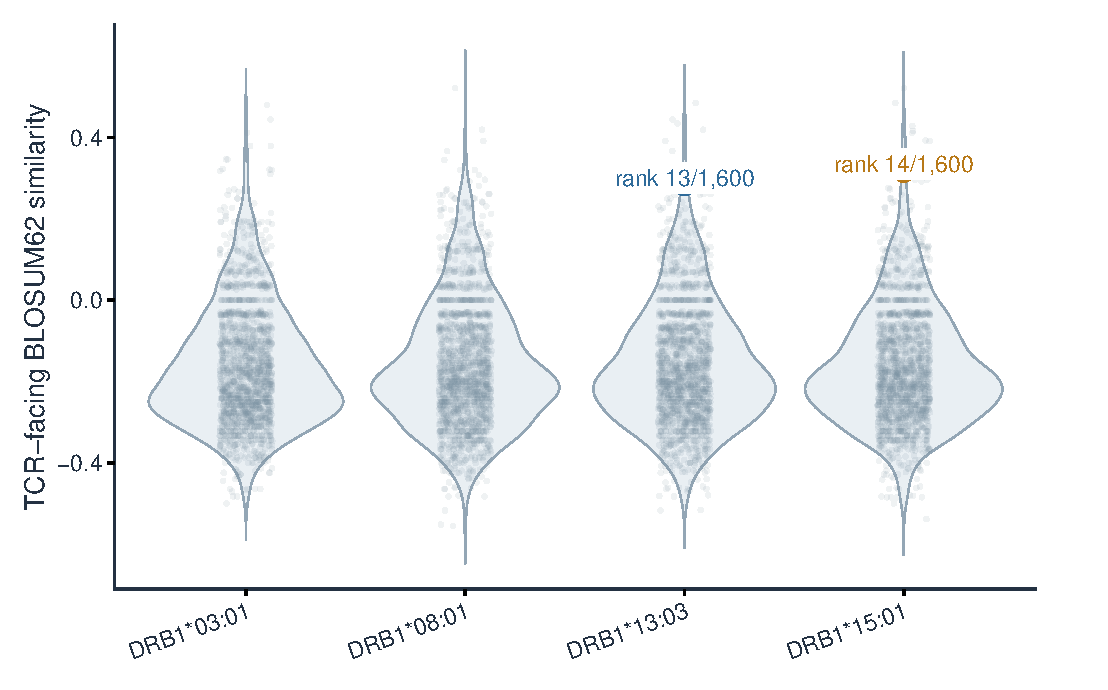
\includegraphics[width=0.95\linewidth]{supplement_figures/figureS1.pdf}
\caption{\textbf{Within-allele distributions of TCR-facing BLOSUM62 similarity scores.} Each point represents one EBV-human peptide comparison ($n=1{,}600$ per HLA allele); violin profiles summarize the allele-specific score distributions. Labels identify the BALF5-TALDO1 pairs selected for evidence review. Reported ranks are calculated within each allele, not across the combined 6,400-pair dataset.}
\label{fig:s1}
\end{figure}

\begin{figure}[H]
\centering
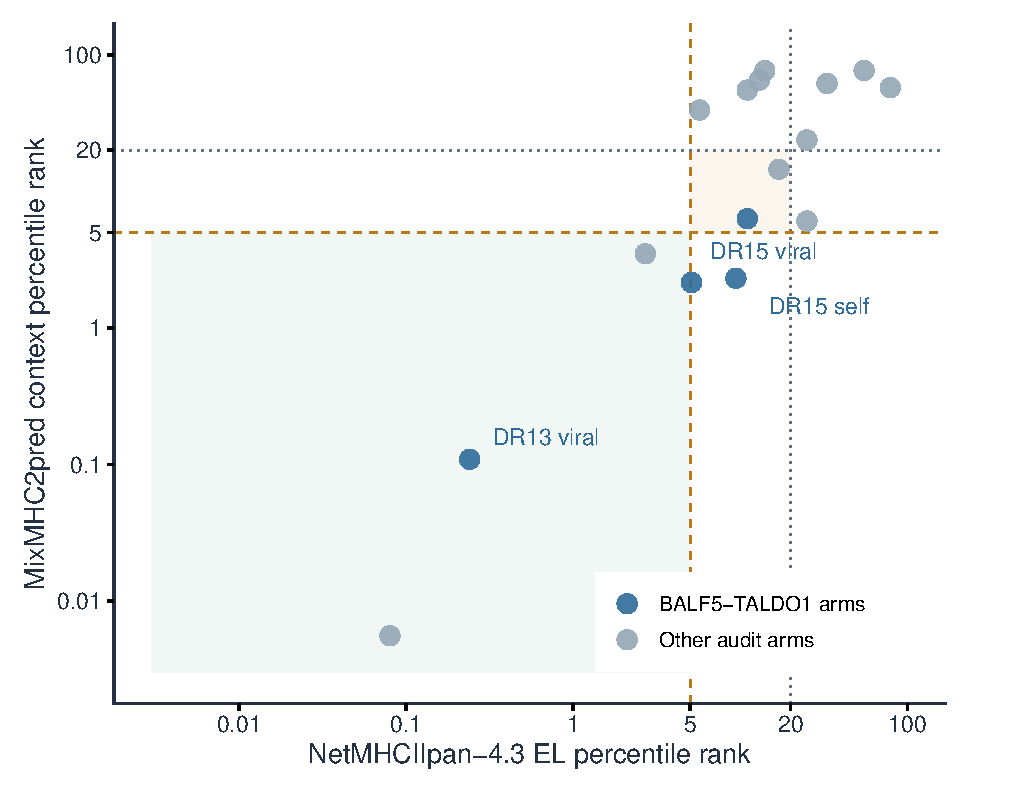
\includegraphics[width=0.92\linewidth]{supplement_figures/figureS2.pdf}
\caption{\textbf{Concordance of peptide-HLA class II binding-percentile predictions in the initial eight-pair audit.} Each point represents one peptide arm. NetMHCIIpan-4.3 EL and MixMHC2pred context percentile ranks are plotted on logarithmic axes; lower values indicate stronger predicted binding. Gold dashed lines mark the $\leq5\%$ full-consensus threshold, gray dotted lines mark the $\leq20\%$ lesser-support threshold, and the shaded region identifies arms below 5\% in both predictors. Blue points are BALF5-TALDO1 arms; gray points are other audited arms.}
\label{fig:s2}
\end{figure}

\section{Supplementary Tables}

\begin{table}[H]\centering\footnotesize
\caption{Top sequence-ranked pairs within each allele.}
\label{tab:s1}
\setlength{\tabcolsep}{3pt}\renewcommand{\arraystretch}{1.2}
\begin{tabular}{p{0.11\textwidth}p{0.28\textwidth}p{0.28\textwidth}p{0.25\textwidth}}
\toprule Allele & Rank 1 & Rank 2 & Rank 3 \\\midrule
*03:01 & \pep{EBNA2}{136-150}-\pep{MOG}{97-109} (0.48) & \pep{BNRF1}{37-51}-\pep{CLDN11}{193-207} (0.44) & \pep{BALF4}{103-116}-\pep{CRYAB}{1-15} (0.41)\\
*08:01 & \pep{EBNA1}{87-101}-\pep{ANO2}{79-93} (0.52) & \pep{BLLF1}{65-75}-\pep{PLP1}{140-152} (0.42) & \pep{BZLF1}{198-210}-\pep{MAG}{612-626} (0.391)\\
*13:03 & \pep{EBNA3B}{139-153}-\pep{MOG}{221-235} (0.49) & \pep{BNRF1}{37-51}-\pep{CLDN11}{193-207} (0.44) & \pep{BARF1}{1-15}-\pep{MAG}{1-15} (0.44)\\
*15:01 & \pep{EBNA1}{87-101}-\pep{ANO2}{79-93} (0.52) & \pep{EBNA3B}{139-153}-\pep{MOG}{221-235} (0.49) & \pep{BALF4}{575-589}-\pep{CNP}{1-15} (0.43)\\\bottomrule
\end{tabular}\end{table}

\begin{table}[H]
\centering
\small
\caption{Initial eight-candidate evidence audit.}
\label{tab:s2}
\setlength{\tabcolsep}{4pt}
\renewcommand{\arraystretch}{1.20}
\begin{tabular}{p{0.30\textwidth}>{\centering\arraybackslash}p{0.11\textwidth}>{\centering\arraybackslash}p{0.11\textwidth}>{\centering\arraybackslash}p{0.10\textwidth}>{\centering\arraybackslash}p{0.10\textwidth}>{\centering\arraybackslash}p{0.13\textwidth}}
\toprule
\shortstack[l]{Candidate pair\\HLA context} & \shortstack{Binding\\V / S} & \shortstack{Register\\V / S} & \shortstack{IEDB\\arms} & \shortstack{Ligand\\arms} & \shortstack{Audit\\status} \\
\midrule
EBNA2-MOG\\HLA-DRB1*03:01 & No / Yes & Yes / Yes & 0 & 0 & Hold \\
BARF1-CRYAB\\HLA-DRB1*03:01 & No / No & No / Yes & 0 & 0 & Hold \\
EBNA1-ANO2\\HLA-DRB1*08:01 & No / No & Yes / Yes & 0 & 0 & Hold \\
EBNA-LP-MOG\\HLA-DRB1*08:01 & No / No & No / Yes & 0 & 0 & Hold \\
EBNA3B-MOG\\HLA-DRB1*13:03 & No / No & No / No & 0 & 0 & Hold \\
BALF5-TALDO1\\HLA-DRB1*13:03 & Yes / No & Yes / Yes & 0 & 0 & \shortstack{\textbf{Medium}\\priority} \\
BALF4-CRYAB\\HLA-DRB1*15:01 & Yes / No & Yes / Yes & 1 & 1 & Hold \\
BALF5-TALDO1\\HLA-DRB1*15:01 & No / No & Yes / Yes & 1 & 0 & \shortstack{\textbf{Medium}\\priority} \\
\bottomrule
\end{tabular}

\vspace{3pt}
\parbox{0.94\linewidth}{\footnotesize\textit{Note.} V/S, viral/self peptide arm. Binding: both NetMHCIIpan-4.3 EL and MixMHC2pred ranks $\leq5\%$ for that arm. Register: both predictors selected the same declared P1-P9 core. IEDB and ligand entries are numbers of peptide arms with exact-HLA supporting records (0-2); they are not numbers of studies or patients. These fields do not establish natural presentation or T-cell cross-reactivity.}
\end{table}

\begin{table}[H]\centering\scriptsize
\caption{Secondary provisional classifications in the 49-pair cohort.}
\label{tab:s3}
\setlength{\tabcolsep}{2pt}\renewcommand{\arraystretch}{1.2}
\begin{tabular}{p{0.13\textwidth}p{0.22\textwidth}p{0.12\textwidth}p{0.23\textwidth}p{0.23\textwidth}}
\toprule Target allele & Viral-human pair & Status & Supporting factor & Limitation \\\midrule
DRB1*15:01 & \pep{BALF5}{627-641}-\pep{TALDO1}{216-230} & Strong-medium & Complete computational consensus; viral IEDB binding & Register instability; no self-arm elution record\\
DRB1*13:03 & \pep{BALF5}{627-641}-\pep{TALDO1}{108-122} & Weak-medium & Expanded binding and register criteria & No verified public record\\
DRB1*15:01 & \pep{EBNA1}{87-101}-\pep{MBP}{217-233} & Weak-medium & Declared register retained across calibrated PANDORA templates & Binding-predictor discrepancy; lower rank\\
DRB1*15:01 & \pep{BALF4}{103-116}-\pep{CRYAB}{1-15} & Strong-low & Initial sequence similarity & Template discordance and register sensitivity\\
DRB1*03:01 & \pep{EBNA2}{136-150}-\pep{MOG}{97-109} & Strong-low & Initial sequence rank & No same-allele PANDORA calibration\\
DRB1*08:01 & \pep{BHRF1}{122-133}-\pep{ANO2}{104-118} & Strong-low & Initial sequence rank & No same-allele PANDORA calibration\\
DRB1*08:01 & \pep{EBNA1}{87-101}-\pep{ANO2}{79-93} & Strong-low & Initial sequence rank & No same-allele PANDORA calibration\\
Various & Various & Untiered & Heterogeneous profiles & Incomplete consensus or evidence\\\bottomrule
\end{tabular}\end{table}

\begin{table}[H]
\centering
\scriptsize
\caption{Constrained-null simulation results for the eight audited pairs. Ten thousand replicates were completed independently for each allele at random seed 20260914. The 95\% null interval reports the 2.5th and 97.5th percentiles.}
\label{tab:s4}
\setlength{\tabcolsep}{3pt}
\renewcommand{\arraystretch}{1.18}
\resizebox{\textwidth}{!}{%
\begin{tabular}{lllrrrrrr}
\toprule
Target & Allele & Pair & \shortstack{Observed\\score (rank)} & \shortstack{Null\\median} & 95\% null interval & \shortstack{Monte Carlo\\$p$} & BH $q$ & maxT $p$ \\
\midrule
HY03\_SEQ\_01 & DRB1*03:01 & EBNA2-MOG & 0.48000 (1) & -0.18519 & [-0.35714, 0.28000] & 0.00790 & 0.06319 & 0.83572 \\
HY03\_SEQ\_02 & DRB1*03:01 & BARF1-CRYAB & 0.27273 (13) & -0.17949 & [-0.32500, 0.34375] & 0.08189 & 0.08189 & 1.00000 \\
HY08\_SEQ\_01 & DRB1*08:01 & EBNA1-ANO2 & 0.52174 (1) & 0.00000 & [-0.32000, 0.52174] & 0.03420 & 0.07199 & 0.66483 \\
HY08\_SEQ\_02 & DRB1*08:01 & EBNA-LP-MOG & 0.32000 (6) & -0.11538 & [-0.46154, 0.32000] & 0.06539 & 0.07634 & 1.00000 \\
HY13\_SEQ\_01 & DRB1*13:03 & EBNA3B-MOG & 0.48485 (1) & -0.13514 & [-0.32432, 0.48485] & 0.03600 & 0.07199 & 0.82102 \\
HY13\_SEQ\_02 & DRB1*13:03 & BALF5-TALDO1 & 0.28125 (13) & -0.15625 & [-0.33333, 0.25806] & 0.01720 & 0.06879 & 1.00000 \\
HY15\_SEQ\_01 & DRB1*15:01 & BALF4-CRYAB & 0.41176 (5) & -0.10000 & [-0.30233, 0.47059] & 0.05559 & 0.07634 & 0.98260 \\
HY15\_SEQ\_02 & DRB1*15:01 & BALF5-TALDO1 & 0.31429 (14) & 0.05714 & [-0.18919, 0.41176] & 0.06679 & 0.07634 & 1.00000 \\
\bottomrule
\end{tabular}%
}

\vspace{3pt}
\begin{minipage}{0.98\textwidth}\footnotesize
Sequence-score calibration only; not evidence of endogenous presentation, pMHC stability, TCR recognition, cross-reactivity, molecular mimicry, or an MS mechanism.
\end{minipage}
\end{table}

\FloatBarrier
\begin{thebibliography}{99}
\bibitem{bjornevik} Bjornevik K, Cortese M, Healy BC, et al. Longitudinal analysis reveals high prevalence of Epstein-Barr virus associated with multiple sclerosis. \textit{Science}. 2022;375:296-301. \url{https://doi.org/10.1126/science.abj8222}
\bibitem{ninds} National Institute of Neurological Disorders and Stroke. \textit{Multiple Sclerosis: Hope Through Research}. \url{https://www.ninds.nih.gov/health-information/disorders/multiple-sclerosis}
\bibitem{lanz} Lanz TV, Brewer RC, Ho PP, et al. Clonally expanded B cells in multiple sclerosis bind EBV EBNA1 and GlialCAM. \textit{Nature}. 2022;603:321-327. \url{https://doi.org/10.1038/s41586-022-04432-7}
\bibitem{iedb} Vita R, et al. The Immune Epitope Database (IEDB): 2024 update. \textit{Nucleic Acids Research}. 2025;53:D436-D443. \url{https://doi.org/10.1093/nar/gkae1092}
\bibitem{uniprot} The UniProt Consortium. UniProt: the Universal Protein Knowledgebase in 2025. \textit{Nucleic Acids Research}. 2025;53:D609-D617. \url{https://doi.org/10.1093/nar/gkae1010}
\bibitem{netmhc} Nilsson JB, Kaabinejadian S, Yari H, et al. Accurate prediction of HLA class II antigen presentation across all loci using tailored data acquisition and refined machine learning. \textit{Science Advances}. 2023;9:adj6367. \url{https://doi.org/10.1126/sciadv.adj6367}
\bibitem{mix2019} Racle J, Michaux J, Rockinger GA, et al. Robust prediction of HLA class II epitopes by deep motif deconvolution of immunopeptidomes. \textit{Nature Biotechnology}. 2019;37:1283-1286. \url{https://doi.org/10.1038/s41587-019-0289-6}
\bibitem{blosum} Henikoff S, Henikoff JG. Amino acid substitution matrices from protein blocks. \textit{PNAS}. 1992;89:10915-10919. \url{https://doi.org/10.1073/pnas.89.22.10915}
\bibitem{grantham} Grantham R. Amino acid difference formula to help explain protein evolution. \textit{Science}. 1974;185:862-864. \url{https://doi.org/10.1126/science.185.4154.862}
\bibitem{af3} Abramson J, Adler J, Dunger J, et al. Accurate structure prediction of biomolecular interactions with AlphaFold 3. \textit{Nature}. 2024;630:493-500. \url{https://doi.org/10.1038/s41586-024-07487-w}
\bibitem{lang} Lang HLE, Jacobsen H, Ikemizu S, et al. A functional and structural basis for TCR cross-reactivity in multiple sclerosis. \textit{Nature Immunology}. 2002;3:940-943. \url{https://doi.org/10.1038/ni835}
\bibitem{apbs} Jurrus E, Engel D, Star K, et al. Improvements to the APBS biomolecular solvation software suite. \textit{Protein Science}. 2018;27:112-128. \url{https://doi.org/10.1002/pro.3280}
\bibitem{dockq} Basu S, Wallner B. DockQ: A quality measure for protein-protein docking models. \textit{PLOS ONE}. 2016;11:e0161879. \url{https://doi.org/10.1371/journal.pone.0161879}
\bibitem{capri} Collins KW, Copeland MM, Brysbaert G, et al. CAPRI-Q: The CAPRI resource evaluating the quality of predicted structures of protein complexes. \textit{Journal of Molecular Biology}. 2024;436:168540. \url{https://doi.org/10.1016/j.jmb.2024.168540}
\bibitem{tcr} Yin R, Ribeiro-Filho HV, Lin V, et al. TCRmodel2: high-resolution modeling of T cell receptor recognition using deep learning. \textit{Nucleic Acids Research}. 2023;51:W569-W576. \url{https://doi.org/10.1093/nar/gkad356}
\bibitem{pride} Perez-Riverol Y, et al. The PRIDE database at 20 years: 2025 update. \textit{Nucleic Acids Research}. 2025;53:D543-D551. \url{https://doi.org/10.1093/nar/gkae1011}
\bibitem{pandora} Parizi FM, Marzella DF, Ramakrishnan G, et al. PANDORA v2.0: Benchmarking peptide-MHC II models and software improvements. \textit{Frontiers in Immunology}. 2023;14:1285899. \url{https://doi.org/10.3389/fimmu.2023.1285899}
\bibitem{modeller} Sali A, Blundell TL. Comparative protein modelling by satisfaction of spatial restraints. \textit{Journal of Molecular Biology}. 1993;234:779-815. \url{https://doi.org/10.1006/jmbi.1993.1626}
\bibitem{thomas} Thomas OG, Rykaczewska U, Galešić M, et al. Anoctamin-2-specific T cells link Epstein-Barr virus to multiple sclerosis. \textit{Cell}. 2026;189:585-602.e38. \url{https://doi.org/10.1016/j.cell.2025.12.032}
\bibitem{hansen} Hansen BE, Rasmussen AH, Jakobsen BK, Ryder LP, Svejgaard A. Extraordinary cross-reactivity of an autoimmune T-cell receptor recognizing specific peptides both on autologous and on allogeneic HLA class II molecules. \textit{Tissue Antigens}. 2007;70:42-52. \url{https://doi.org/10.1111/j.1399-0039.2007.00849.x}
\bibitem{brown} Brown JH, Jardetzky TS, Gorga JC, et al. Three-dimensional structure of the human class II histocompatibility antigen HLA-DR1. \textit{Nature}. 1993;364:33-39. \url{https://doi.org/10.1038/364033a0}
\bibitem{sewell} Sewell AK. Why must T cells be cross-reactive? \textit{Nature Reviews Immunology}. 2012;12:669-677. \url{https://doi.org/10.1038/nri3279}
\bibitem{denzin} Denzin LK, Cresswell P. HLA-DM induces CLIP dissociation from MHC class II alpha beta dimers and facilitates peptide loading. \textit{Cell}. 1995;82:155-165. \url{https://doi.org/10.1016/0092-8674(95)90061-6}
\end{thebibliography}

\end{document}
